\documentclass[a4paper]{article}
\usepackage{style}

\title{Robotics\\ Lab 2: Navigation}
\author{Group 3\\Sebastian Grasdijk (s1972243) \& Niels Kluiter (s2225328)}

\newcommand*\rfrac[2]{{}^{#1}\!/_{#2}}

% TODOs
\usepackage{todonotes}

\begin{document}

\maketitle

\noindent The code for this assignment can be found in the branch \t{group3}, it is tagged in the package \t{navigation}. We do have a small side note, which we unfortunately were unable to correct. Our code all ran fine, but after we used Alice some of the code appeared to have broken due to package changes or something. We have added the working code as a zip with the report, but it might be different than what currently is on our git branch.

We apologise for the inconvience, we attempted to correct it on thursday but the lab was closed at the time.

\section*{Exercise 1}
 %!TEX root = report.tex

\subsection*{1.a}
For the assignment a launch file has to be created using Gmapping and teleoperation, which would finally save the map. The launch file is as follows:

\lstinputlisting[
	caption={The launch file to map the room.},
	label={lst:1:teleopMap}, 
	language=Python,
	float
]{./src/1/create_map.launch}

In order to get a map, the following commands have to be used in different terminals:

\begin{lstlisting}
	roslaunch navigation exercise1.launch
	roslaunch navigation create_map
\end{lstlisting}

\begin{itemize}
	\item \todo[inline]{De transforms gebeuren automagisch op basis van URDF, noem welke het zijn. zie GMapping wiki.}
\end{itemize}

\begin{figure}
	\centering
	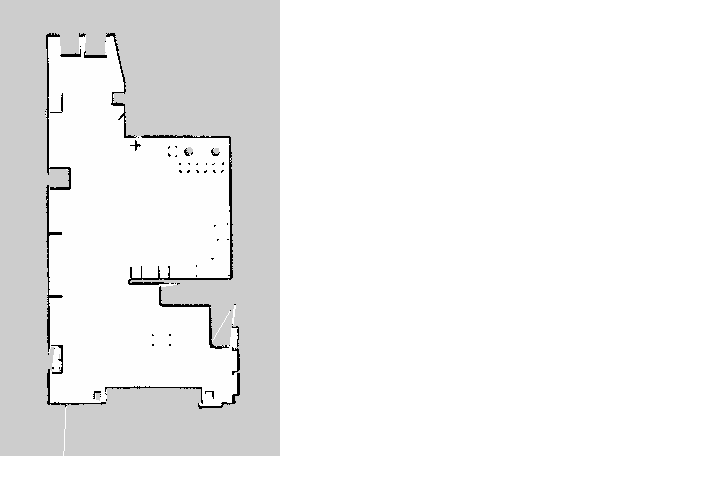
\includegraphics[width=\textwidth]{./img/map_teleop.png}
	\caption{The map that was made through mapping with teleop keyboard package.}
	\label{fig:1:map}
\end{figure}

\subsection*{1.b}

\todo[inline]{How do you run this?!}

For this assignment, the map from the first part had to be reused in Rviz, together with amcl. The following commands were necessary:

\begin{lstlisting}
	roslaunch navigation exercise1.launch
	roslaunch navigation amcl.launch
\end{lstlisting}

This gave a 2D map in Rviz, with an amcl representation of the robot in gazebo, as well as the 3D model in gazebo. In order to try and break the representations of the robot between Rviz and Gazebo, a lot of noise was introduced. Using this meant the rviz robot was at a different point than the gazebo robot after a while.

\lstinputlisting[
	caption={The launch file to map the room.},
	label={lst:2:teleopAmcl}, 
	language=Python,
	float
]{./src/1/amcl.launch}

\todo[inline]{add code to change location through python}
\todo[inline]{change speeds on robot}
\todo[inline]{show difference gazebo/rviz}

\section*{Exercise 2}
%!TEX root = report.tex

For this exercise we created a launch file, which launches the Alice simulation, the visualisation of the situation in Rviz and the navigation stack, which is defined by a second launch file.

\lstinputlisting[
	caption={The launch file for the entire exercise \t{exercise2.launch}.},
	label={lst:2:exercise}, 
	language=XML
]{./src/2/exercise2.launch}

This file can launched using the following command

\begin{lstlisting}
	roslaunch navigation exercise2.launch
\end{lstlisting}

The launch file that defines the navigation file and the parameter files that it includes can be found in \cref{sec:a:ass2}, the interesting parts of these are explained below:

The first parameter we set is the \t{controller\_frequency} this is the frequency (in Hertz) at which velocity commands are sent to the robot base, this is 10 Hz for our navigation stack:

\lstinputlisting[
	caption={The controller frequency},
	label={lst:2:c_freq}, 
	language=XML,
	firstline=37,
	lastline=37
]{./src/2/alice_nav.launch}

Before moving to a location, \t{move\_base} has to find a path to this location, but sometimes a path cannot be found, the \t{planner\_patience} parameter tells how many seconds \t{move\_base} should keep trying to find a path to a certain location, before moving on. In our case this is 3 seconds:

\lstinputlisting[
	caption={The planner patience},
	label={lst:2:p_pat}, 
	language=XML,
	firstline=39,
	lastline=39
]{./src/2/alice_nav.launch}

Furthermore, once a plan has been made, velocities have to be determined for the robot to move. This can fail too. The \t{controller\_patience} determines how many seconds \t{move\_base} should wait for velocity controls, before failing. For this parameter we use 10 seconds.

\lstinputlisting[
	caption={The controller patience},
	label={lst:2:c_pat}, 
	language=XML,
	firstline=40,
	lastline=40
]{./src/2/alice_nav.launch}

If the robot has to wait longer than set in the patience parameter, it is stuck. At this point it will start doing its recovery behaviours. The \t{clearing\_rotation\_allowed} parameter tells if the robot is allowed to rotate on spot if this happens. In our stack the robot is not:

\lstinputlisting[
	caption={Rotating on spot recovery is not allowed},
	label={lst:2:rotate}, 
	language=XML,
	firstline=38,
	lastline=38
]{./src/2/alice_nav.launch}

Another recovery behaviour is clearing the robots costmaps, the costmap of a robot determines where the robot can safely move. Costmaps are constantly updated and can thus cause a robot to get stuck. In our case the robot is allowed to clear costmaps as a recovery behaviour. The recovery behaviours that a robot does use, are defined by the \t{recovery\_behaviors} parameter. This parameter can be set directly from the launch file, like the parameters before, or from yaml files containing more specific parameters for certain parts of the navigation stack, we set the \t{recovery\_parameters} parameter from the \t{costmap_common_params.yaml} file specifying the parameters that are common among our local and global planners:

\lstinputlisting[
	caption={Use clearing costmaps as recovery behaviour},
	label={lst:2:clear}, 
	language=XML,
	firstline=5,
	lastline=8
]{./src/2/costmap_common_params.yaml}

The files yaml files containing the specific parameters are included from the navigation stack launch file:

\lstinputlisting[
	caption={Include YAML files containing more parameters},
	label={lst:2:yaml}, 
	language=XML,
	firstline=25,
	lastline=35
]{./src/2/alice_nav.launch}

The calculation of a path, as mentioned above, is done by a module called the global planner. The global planner uses shortest path algorithms like Dijkstra and A* to find a path through its costmap with the lowest possible cost. Once a path is calculated, a local planner with repeatedly try to determine what to do to follow this plan. It will simulate trajectories for many different velocities and then chooses the velocities that will get the robot to its destination the fastest, without hitting obstacles or moving too far away from the plan. The default planners used in ROS are the Navfn global planner and the Trajectory Rollout local planner, which simulates over a larger period than the other common choice: Dynamic Window Approach. This might result in a slightly better performance. The navigation stack in this exercise uses these default planners, so parameters for this need not be set. Other planners could however be chosen using the \t{base\_global\_planner} and \t{base\_local\_planner} parameters.

The costmaps that the planners use, are updated while the robot is moving. It is possible to shut this down when the robot is in an inactive. By default the costmaps are not shut down, but we enabled it by adding the following parameter:

\lstinputlisting[
	caption={Shutdown costmaps in an inactive state},
	label={lst:2:shutdown}, 
	language=XML,
	firstline=43,
	lastline=43
]{./src/2/alice_nav.launch}

Costmaps are used to check how big the risk of collision is when planning, to do this a footprint of the robot is needed to see which parts of the costmaps it covers at each moment. This footprint needs to be convex to be able to do the right calculations. Each of the planners uses an own costmap. For the global planner we used a footprint that is circular, defined by setting a \t{robot\_radius} in our \t{global_costmap_params.yaml}  file.

\lstinputlisting[
	caption={Global footprint},
	label={lst:2:global_footprint}, 
	language=XML,
	firstline=4,
	lastline=4
]{./src/2/global_costmap_params.yaml}

For the local planner we used a rectangular footprint, representing the rectangular base of the robot itself. It is set by the \t{footprint} parameter in \t{local_costmap_params.yaml}:

\lstinputlisting[
	caption={Local footprint},
	label={lst:2:local_footprint}, 
	language=XML,
	firstline=14,
	lastline=15
]{./src/2/local_costmap_params.yaml}

Higher costs in costmaps are caused by proximity to objects, how close the robot needs to be for costs to go up is set by \t{inflation_radius} parameter, these can be different between the two planners, we set inflation radius for the local costmap 10 centimetres higher than that of the global costmap:

\lstinputlisting[
	caption={Global inflation radius},
	label={lst:2:global_inflation}, 
	language=XML,
	firstline=19,
	lastline=19
]{./src/2/global_costmap_params.yaml}

\lstinputlisting[
	caption={Local inflation radius},
	label={lst:2:local_inflation}, 
	language=XML,
	firstline=23,
	lastline=23
]{./src/2/local_costmap_params.yaml}

To build a costmap we need sensors to detect obstacles, for this Alice uses Xtions and lasers. These have to be set in the parameters, we set this in the file \t{costmap_common_params.yaml} that defines parameters shared between the global and local costmaps:

\lstinputlisting[
	caption={Defining sensors},
	label={lst:2:sensor_def}, 
	language=XML,
	firstline=10,
	lastline=17
]{./src/2/costmap_common_params.yaml}

These sensors then have to be enabled in the planners, these lines can be found in both the global costmap parameters and the local costmap parameters.

\lstinputlisting[
	caption={Enabling sensors},
	label={lst:2:sensor_enable}, 
	language=XML,
	firstline=25,
	lastline=33
]{./src/2/local_costmap_params.yaml}

The only difference between the local and the global parameters here is the \t{combination_method} parameter. This set for the local costmap to be 0, meaning that the Xtions have a higher priority than the lasers (1) in the local planner. This is not present in the global parameters.



\section*{Exercise 3}
%!TEX root = report.tex

We created our own behavior called \t{movetolocation}, in which the program received text input, for which it then had to give adequate feedback. We used the NLP class, which was meant for assignment 4, for this assignment already, in order to reduce the complexity of the sentences. This made them easier to parse, meaning less text had to be hard-coded.

\lstinputlisting[
	caption={The formulation of the response.},
	label={code:3}, 
	language=python,
	firstline=28,
	lastline=48
]{./src/movetolocation_0.py}

The response is formulated in \cref{code:3}, where the class NLP is also called. The optionals as well as any potential names are first removed in order to reduce the complexity of the message that has to be parsed. 

Afterwards the sentence is checked if there are tokens like \t{<verb>} or \t{<location>} present. If they aren't, then an if sentence == x, reply y system is used. If there are tokens present, then the sentence gets split in the respective words. 

If a verb is found from the dictionary, then the location is retrieved and the robot responses that he will move to the location. If it can't find a verb from the dictionary, then from the list of sentences it should be able to respond to, there is only one option left, a request to reach the dining table. Then that is the final response.

\lstinputlisting[
	caption={The grammar used},
	label={grammar}, 
	language=XML,
]{./src/NielsSebastiaan.gram}

The grammar used can be seen in \cref{grammar}. To make the grammar easily usable for the NLP class, have we named the verbs \t{<verb>} and names with \t{<start}. The sentences are hardcoded due to their lack of overlap with the other sentences that the program had to be able to respond to.

Launch instructions:
\begin{lstlisting}
$ roscore
$ ./start.sh config/assignment3
$ python speech/speech_to_memory.py "hyp1"
\end{lstlisting}

\section*{Exercise 4}
%!TEX root = report.tex
To be able to deal with uncertainty, we modified the behavior used in exercise 3. We replaced the \t{formulate_response} function by a similar response generation from the NLP class that is able to deal with uncertainty. We modified the original NLP class to one that is able to deal with our grammar.
The first thing that happens in our NLP class is checking if there are elements in a hypothesis that correspond to our grammar. It does this for the two best hypotheses separately. The NLP uses some symbols directly from the grammar for parsing, like \t{<start>}, \t{<verb>}, \t{<location>} and \t{<sentence>}. Using these symbols, the class is able to determine whether an hypothesis is a question, an order to navigate or not anything corresponding to the grammar at all. The main elements, like what verb was used, what location was mentioned and what exact question was asked is returned and compared to that of the other hypothesis.
If both hypotheses are equal, an appropriate response is given like in exercise 3:

\begin{lstlisting}[language=bash]
I heard one of these:
what is the oldest most widely used drug on earth
alice what is the oldest most widely used drug on earth

[Alice says] Okay, The oldest, most widely used drug on earth is coffee.
\end{lstlisting}

If hypotheses are unequal the inequality is explored. For example, in a case where both are navigation commands, but there is a difference in locations, the class asks the user to repeat the desired destination:

\begin{lstlisting}[language=bash]
I heard one of these:
alice navigate to the living room
go to the kitchen

living room
kitchen
[Alice says] Where did you want me to navigate?
> kitchen
[Alice says] Okay, I will go to the kitchen
\end{lstlisting}

When there are two unequal questions the system asks the user to repeat the question:

\begin{lstlisting}[language=bash]
[Alice says] Okay, The oldest, most widely used drug on earth is coffee.
I heard one of these:
alice what time is it
alice who are your creators

[Alice says] could you repeat your question?
> what time is it
[Alice says] Okay, The current time is: 18:09:29.
\end{lstlisting}

We were able to test this NLP class on it's own and write code that connects this to our behavior. However due to time constraints we were not able to test this as an actual behavior on the robot lab systems.

Launch instructions, assuming listing \ref{lst:4:behavior} is used as behavior:
\begin{lstlisting}
$ roscore
$ ./start.sh config/assignment3
$ python speech/speech_to_memory.py "hyp1" ["hyp2"]
\end{lstlisting}

\section*{Exercise 5}
%!TEX root = report.tex


\section*{Exercise 6}
%!TEX root = report.tex

\begin{lstlisting}
	roslaunch alice_gazebo alice_simulation.launch	
	roslaunch navigation exercise4.launch
	rosrun navigation print_something.py
\end{lstlisting}

The same robot model was used as in assignment 4, with the exception that a subscriber node listens to whether the goal was reached and when it is reached, that it then prints whether the goal is reached or not. If the goal has failed to have been reached for 3 times, then the goal gets cancelled, as seen in \cref{lst:1:sub}.

\lstinputlisting[
	caption={The subscriber node},
	label={lst:1:sub}, 
	language=Python,
]{./src/6/print_something.py}

\section*{Exercise 7}
%!TEX root = report.tex

 \todo[inline]{How do you run this?!}

\begin{figure}
	\centering
	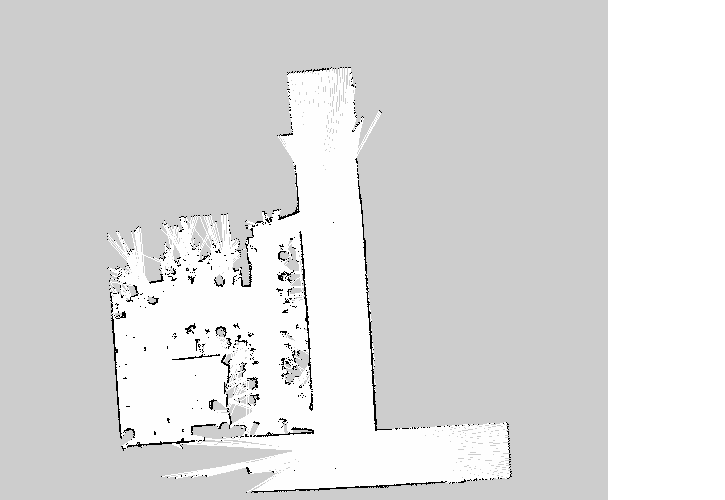
\includegraphics[width=\textwidth]{./img/real_lab.png}
	\caption{The map that was made of the lab through mapping with teleop keyboard package.}
	\label{fig:1:map}
\end{figure}

\printbibliography

\clearpage
\appendix
%!TEX root = report.tex
\section{Assignment 1}
\label{sec:a:ass1}
% \lstinputlisting[
% 	caption={The file \t{assignment.urdf.xacro}.}, 
% 	label={lst:2:ass1}, 
% 	language=XML
% ]{./src/2/assignment.urdf.xacro.xml}

\end{document}